\documentclass[10pt,A4]{article}	
\usepackage[utf8]{inputenc}

%----------------------------------------------------------------------------------------
%	LOGIC
%----------------------------------------------------------------------------------------

% provides \isempty test
\usepackage{xstring, xifthen}

%----------------------------------------------------------------------------------------
%	FONT BASICS
%----------------------------------------------------------------------------------------

\usepackage[default]{raleway}

% set font default
\renewcommand*\familydefault{\sfdefault} 	
\usepackage[T1]{fontenc}

%----------------------------------------------------------------------------------------
%	PAGE LAYOUT  DEFINITIONS
%----------------------------------------------------------------------------------------

% page outer frames (debug-only)
% \usepackage{showframe}	

% we use paracol to display breakable two columns
\usepackage{paracol}

\usepackage[a4paper]{geometry}
\geometry{top=1cm, bottom=1cm, left=0.5cm, right=0.5cm}

\usepackage{fancyhdr}
\pagestyle{empty}

% space between header and content
% \setlength{\headheight}{0pt}

% indentation is zero
\setlength{\parindent}{0mm}

%----------------------------------------------------------------------------------------
%	TABLE /ARRAY DEFINITIONS
%---------------------------------------------------------------------------------------- 

% extended aligning of tabular cells
\usepackage{array}

% custom column right-align with fixed width
% use like p{size} but via x{size}
\newcolumntype{x}[1]{%
>{\raggedleft\hspace{0pt}}p{#1}}%

%----------------------------------------------------------------------------------------
%	GRAPHICS DEFINITIONS
%---------------------------------------------------------------------------------------- 

%for header image
\usepackage{graphicx}

%for drawing graphics		
\usepackage{tikz}				
\usetikzlibrary{shapes, backgrounds, mindmap, trees}
	
%----------------------------------------------------------------------------------------
%	GLOBAL VARIBLES
%----------------------------------------------------------------------------------------

%----------------------------------------------------------------------------------------
%	Color DEFINITIONS
%---------------------------------------------------------------------------------------- 
\usepackage{transparent}
\usepackage{color}

% primary color
\definecolor{maincol}{RGB}{ 225, 0, 0 }

% accent color, secondary
% \definecolor{accentcol}{RGB}{ 250, 150, 10 }

% dark color
\definecolor{darkcol}{RGB}{ 70, 70, 70 }

% light color
\definecolor{lightcol}{RGB}{245,245,245}

%----------------------------------------------------------------------------------------
%   Profile
%----------------------------------------------------------------------------------------

\newcommand{\gfullname}{Nguyen Hoang Nam}
\newcommand{\gaddress}{2F 14 Street, District 7, HCM}
\newcommand{\gphone}{+84 90 236 59 38}
\newcommand{\gmail}{nguyenhoangnam.dev@gmail.com}
\newcommand{\ggithub}{Nguyen-Hoang-Nam}

%----------------------------------------------------------------------------------------
%	UTILS
%----------------------------------------------------------------------------------------

% returns minipage width minus two times \fboxsep
% to keep padding included in width calculations
% can also be used for other boxes / environments
\newcommand{\mpwidth}{\linewidth-\fboxsep-\fboxsep}

%----------------------------------------------------------------------------------------
%	FONT AWESOME ICONS
%----------------------------------------------------------------------------------------

\usepackage{fontawesome}

% use to vertically center content
% credits to: http://tex.stackexchange.com/questions/7219/how-to-vertically-center-two-images-next-to-each-other
\newcommand{\vcenteredinclude}[1]{\begingroup
\setbox0=\hbox{\includegraphics{#1}}
\parbox{\wd0}{\box0}\endgroup}

% use to vertically center content
% credits to: http://tex.stackexchange.com/questions/7219/how-to-vertically-center-two-images-next-to-each-other
\newcommand*{\vcenteredhbox}[1]{
    \begingroup
        \setbox0=\hbox{#1}\parbox{\wd0}{\box0}
    \endgroup
}

% icon shortcut
\newcommand{\icon}[3] { 							
	\makebox(#2, #2){\textcolor{maincol}{\csname fa#1\endcsname}}
}	

% icon with text shortcut
\newcommand{\icontext}[4]{ 						
	\vcenteredhbox{\icon{#1}{#2}{#3}}  \hspace{2pt}  \parbox{0.9\mpwidth}{\textcolor{#4}{#3}}
}

% icon with website url
\newcommand{\iconhref}[5]{ 						
    \vcenteredhbox{\icon{#1}{#2}{#5}}  \hspace{2pt} \href{#4}{\textcolor{#5}{#3}}
}

%============================================================================%
%
%	CV COMMANDS
%
%============================================================================%

%----------------------------------------------------------------------------------------
%	 CV LIST
%----------------------------------------------------------------------------------------

% renders a standard latex list but abstracts away the environment definition (begin/end)
\newcommand{\cvlist}[1] {
	\begin{itemize}{#1}\end{itemize}
}

%----------------------------------------------------------------------------------------
%	 CV TEXT
%----------------------------------------------------------------------------------------

% base class to wrap any text based stuff here. Renders like a paragraph.
% Allows complex commands to be passed, too.
% param 1: *any
\newcommand{\cvtext}[1] {
	\begin{tabular*}{1\mpwidth}{p{0.98\mpwidth}}
		\parbox{1\mpwidth}{#1}
	\end{tabular*}
}

%----------------------------------------------------------------------------------------
%	CV SECTION
%----------------------------------------------------------------------------------------

% Renders a a CV section headline with a nice underline in main color.
% param 1: section title
\newcommand{\cvsection}[1] {
	\vspace{4pt}
	\cvtext{
		\textbf{\Large{\textcolor{darkcol}{\uppercase{#1}}}}\\[-4pt]
		\textcolor{maincol}{ \rule{0.1\textwidth}{2pt} } \\
	}
}

%----------------------------------------------------------------------------------------
%	META SKILL
%----------------------------------------------------------------------------------------

% Renders a progress-bar to indicate a certain skill in percent.
% param 1: name of the skill / tech / etc.
% param 2: level (for example in years)
% param 3: description of skill
\newcommand{\cvskill}[3] {
	\begin{tabular*}{1\mpwidth}{p{0.72\mpwidth}  r}
 		\textcolor{black}{\large{\textbf{#1}}} & \textcolor{maincol}{#2}\\[4pt]
	\end{tabular*}
  	
  	\hspace{4pt}
  	\vspace{8pt}
  	\parbox{0.9\mpwidth}{#3}\\[2pt]
  	
  	\vspace{8pt}
}


%----------------------------------------------------------------------------------------
%	 CV EVENT
%----------------------------------------------------------------------------------------

% Renders a table and a paragraph (cvtext) wrapped in a parbox (to ensure minimum content
% is glued together when a pagebreak appears).
% Additional Information can be passed in text or list form (or other environments).
% the work you did
% param 1: time-frame i.e. Sep 14 - Jan 15 etc.
% param 2:	 event name (job position etc.)
% param 3: Customer, Employer, Industry
% param 4: Short description
\newcommand{\cvevent}[4] {
	
	% we wrap this part in a parbox, so title and description are not separated on a pagebreak
	% if you need more control on page breaks, remove the parbox
	\parbox{\mpwidth}{
		\begin{tabular*}{1\mpwidth}{p{0.20\mpwidth}  l}
	 		{#1} & \large{\textbf{#2}} \\[2pt]
			& \textbf{#3} \\
			& \parbox{0.75\mpwidth}{\small{#4}} \\
		\end{tabular*}\\[6pt]
	}
	\vspace{8pt}
}

\usepackage[hidelinks]{hyperref}

%============================================================================%
%
%
%
%	DOCUMENT CONTENT
%
%
%
%============================================================================%
\begin{document}
\columnratio{0.35}
\setlength{\columnsep}{0.5cm}
\setlength{\columnseprule}{4pt}
\colseprulecolor{lightcol}

\begin{paracol}{2}
\begin{leftcolumn}

%---------------------------------------------------------------------------------------
%	AVATAR
%---------------------------------------------------------------------------------------
\begin{center}
    \begin{tikzpicture}
        \clip circle (2.5cm); 
        \path (0,0) node{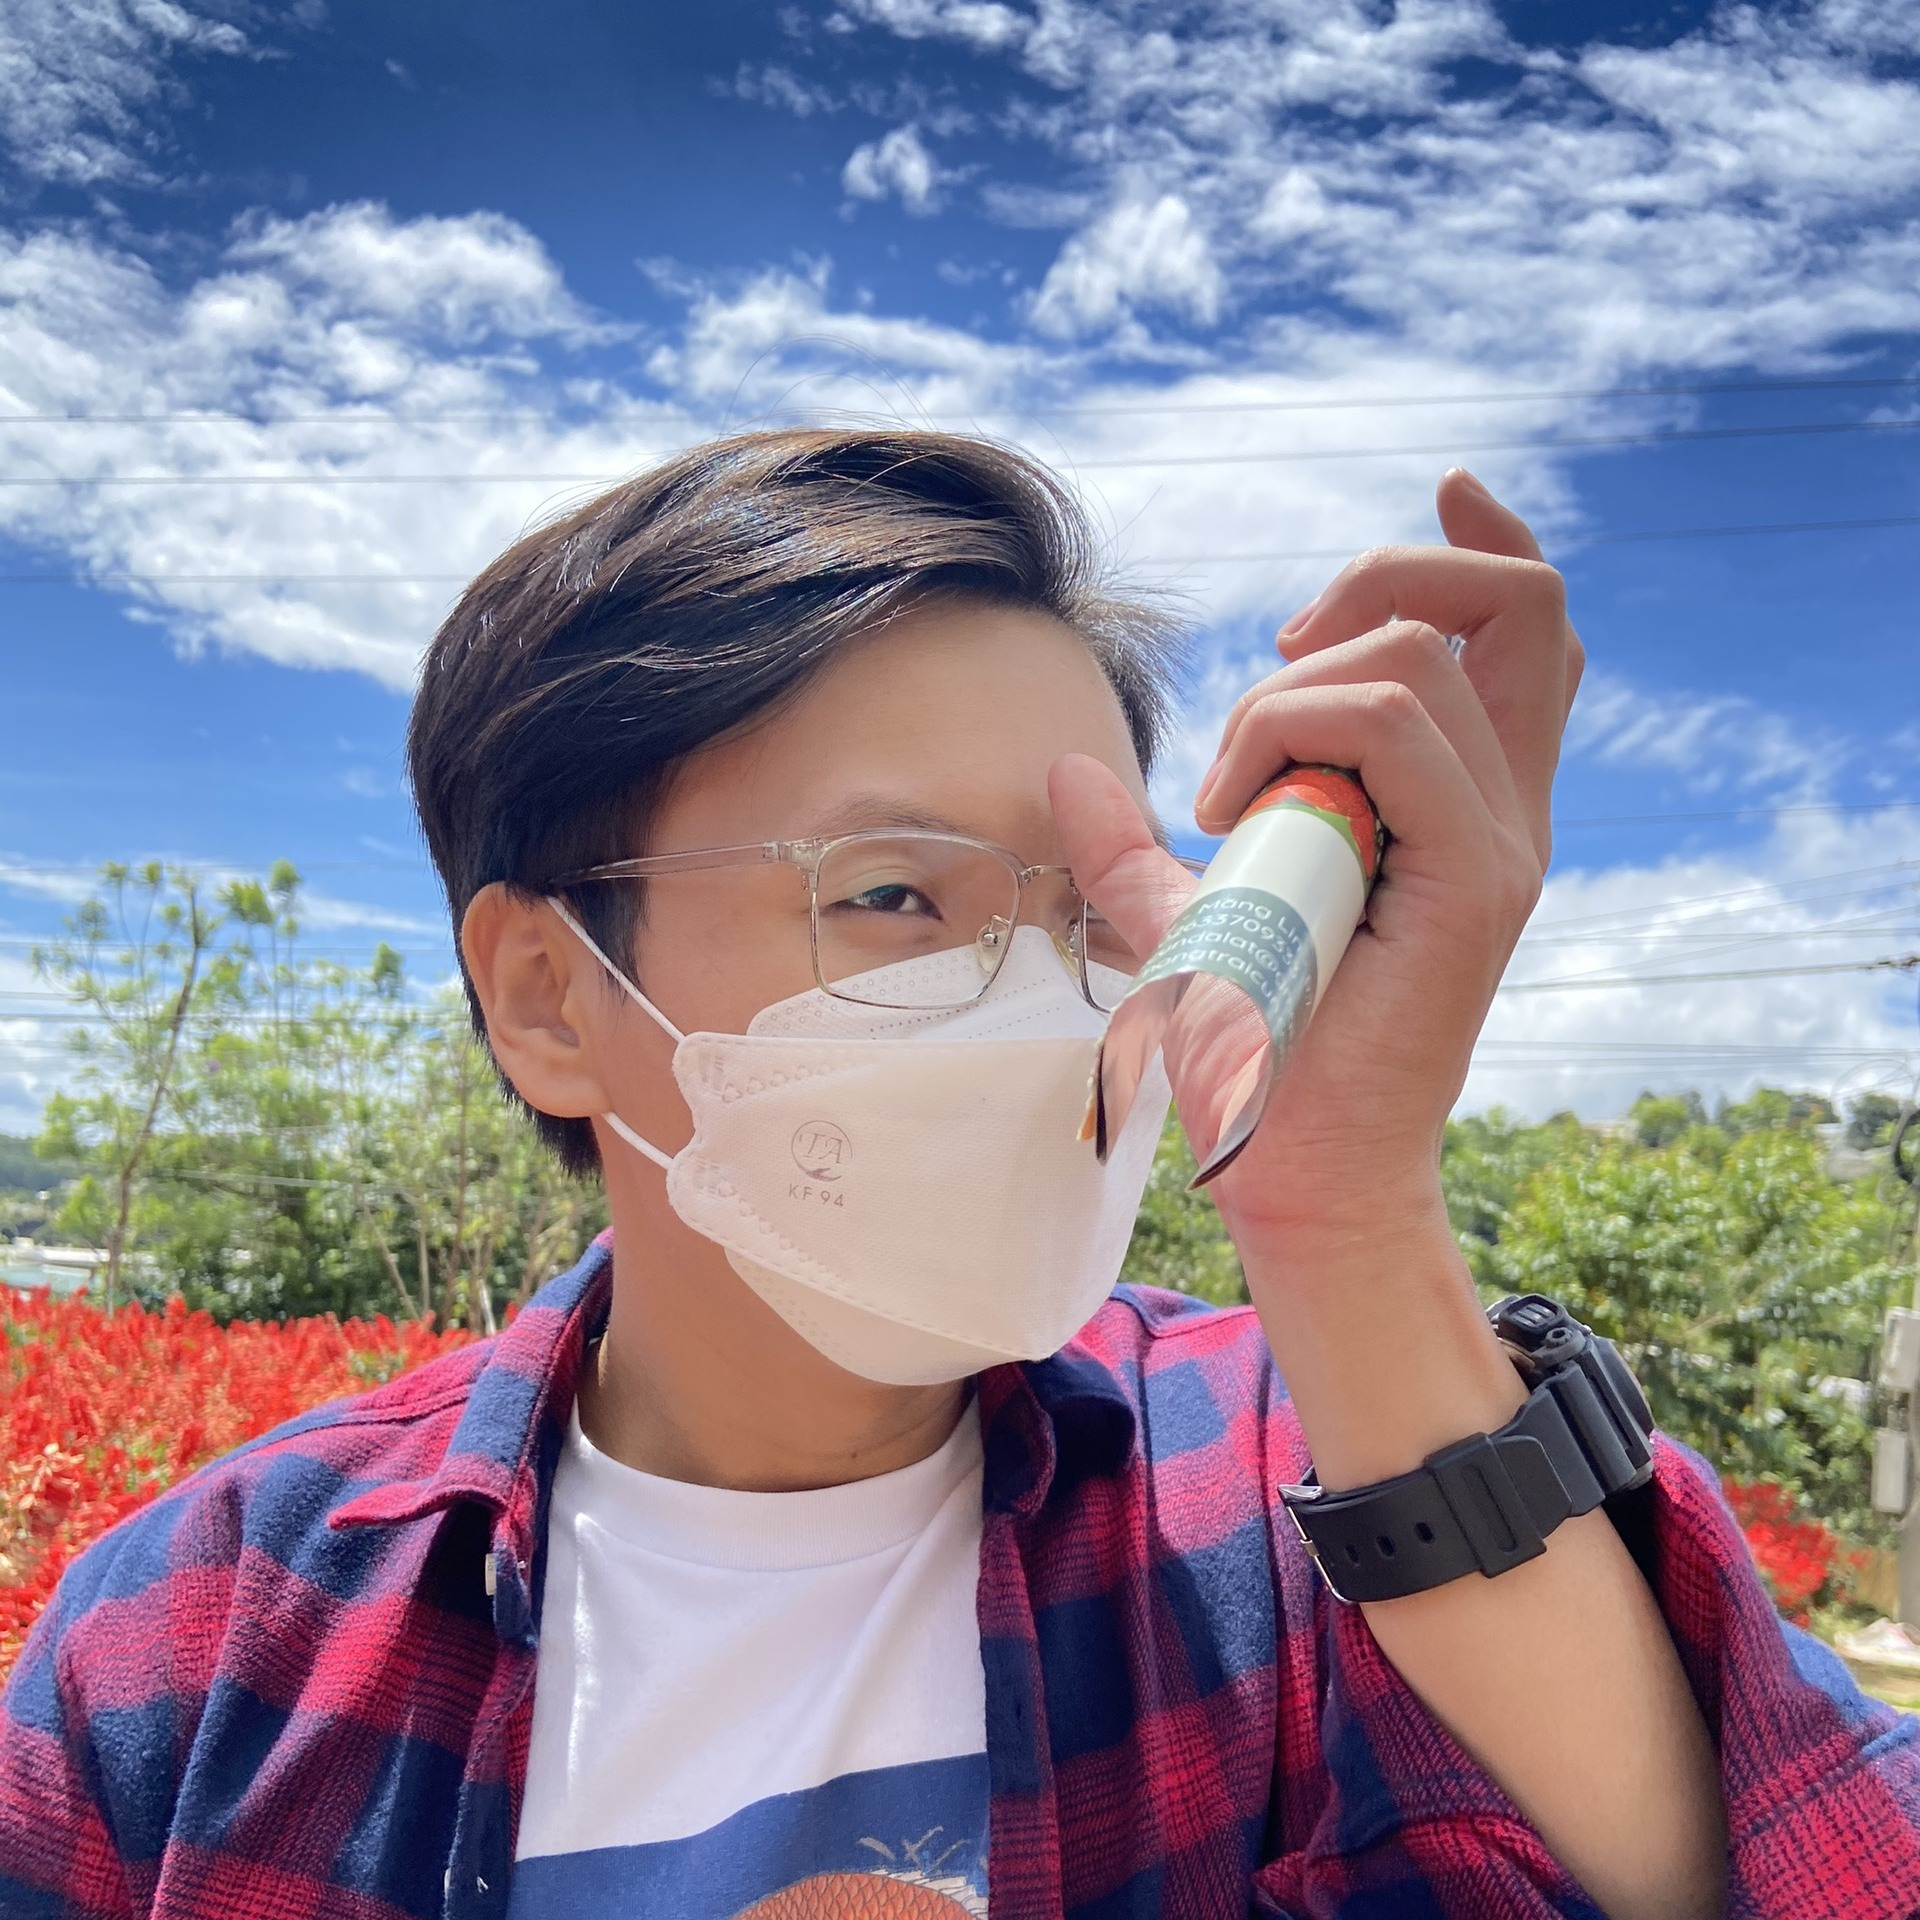
\includegraphics[width=5cm]{avatar.jpg}};
    \end{tikzpicture}
\end{center} 

%---------------------------------------------------------------------------------------
%	PROFILE
%----------------------------------------------------------------------------------------
\begin {center}
	\LARGE{ \textbf{ \uppercase{ \gfullname } } } \\[-10pt]
	\textcolor{red}{ \rule{0.1\textwidth}{1.25pt} } \\[10pt]
	\large{ Frontend and Backend Developer with Three Years of Experience }
\end {center}

\icontext{MapMarker}{12}{\gaddress}{black}\\[6pt]
\icontext{Phone}{12}{\gphone}{black}\\[6pt]
\iconhref{Envelope}{12}{\gmail}{mailto:\gmail}{black}\\[6pt]
\iconhref{Github}{12}{\ggithub}{https://\ggithub}{black}\\[6pt]

%---------------------------------------------------------------------------------------
%	SKILLS
%----------------------------------------------------------------------------------------
\cvsection{SKILLS}

\cvskill{Backend} {2+ yrs} {0.7} {Golang, Rust, NodeJS, Python, GraphQL, gRPC, and ASP.NET core} \\[-2pt]

\cvskill{Database} {2+ yrs} {0.8} {MongoDB, DynamoDB, MySQL, Redis, and Elasticsearch.} \\[-2pt]

\cvskill{Frontend} {3+ yrs} {0.8} {SCSS, WebAssembly, Webpack, React, Svelte, and Tailwind.} \\[-2pt]

\cvskill{Devops tool} {1+ yrs} {0.6} {Docker, Github Action, Husky, Travis CI, and Heroku.} \\[-2pt]

\cvskill{Linux} {1+ yrs} {0.7} {Ubuntu, Neovim, Lua, and Bash.} \\[-2pt]

\end{leftcolumn}
\begin{rightcolumn}

%---------------------------------------------------------------------------------------
%	WORK EXPERIENCE
%----------------------------------------------------------------------------------------
\cvsection{WORK EXPERIENCE}

\cvevent
	{2019}
	{Intern Web Developer}
	{Nhotim company - Information Technology Park}
	{Reviewing ASP.NET MVC 5 legacy code, and having a change to create Socket for chat box component using ASP.NET.}

\cvevent
	{2020}
	{Junior Frontend Developer}
	{ATP company - Pearl Plaza}
	{Starting from scratch to build main landing page, and experiencing with SCSS, Pug, Gulp, PosCSS.}

%---------------------------------------------------------------------------------------
%	EDUCATION
%---------------------------------------------------------------------------------------
% \vfill\null
\cvsection{EDUCATION}

\cvevent
	{2019 - 2022}
	{Bachelor of Computer Vision}
	{University of Science}
	{Having strong knowledge of how computer working, algorithms, object-oriented, designing database. Studying image's processing, classification, tracking, and detection using convolutional neural network, YOLO.}

%---------------------------------------------------------------------------------------
%	PROJECT
%---------------------------------------------------------------------------------------
% \vfill\null
\cvsection{PROJECT}

\cvevent
	{12 - 2019}
	{Draw Geometry}
	{Open Source - Github}
	{Starting from scratch to build drawing application using only jQuery, dealing with legacy javascript framework, and providing well design over other similar product.}
	
\cvevent
	{4 -2020}
	{MySQLoose}
	{Open Source - Github}
	{Creating Object Relational Mapping for MySQL that working exactly like Mongoose, dealing with abstraction of object in javascript, and prevent SQL injection in MySQL's query.}
	
\cvevent
	{6 - 2020}
	{Research Library}
	{Open Source - Github}
	{Dealing with presenting data in academic format, creating network to share document effectively, storing and processing files without bottleneck. Preventing scam, fraud accounts and malware files.}
	
\cvevent
	{3 - 2021}
	{Image Enhancement}
	{Open Source - Github}
	{Implementing lots of image's processing algorithms for image enhancement, increasing contrast, equalizing color.}
	
\cvevent
	{5 - 2021}
	{Let Shorten}
	{Open Source - Github}
	{Building with performance in mind, backend is supported by Golang, DynamoDB, Redis, Elasticsearch, and frontend is run by Svelte, TailwindCSS. Moreover, technical stack can effectively scale horizontal with zero downtime.}


\end{rightcolumn}
\end{paracol}
\end{document}

